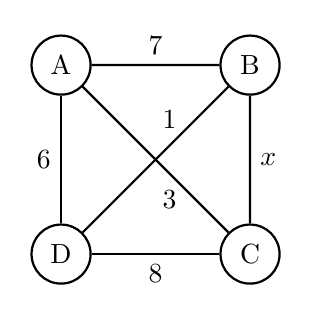
\begin{tikzpicture}[scale=1.2, >=stealth]
    \node[circle, draw, thick, minimum size=7.5mm, inner sep=0pt] (A) at (0, 2) {A};
    \node[circle, draw, thick, minimum size=7.5mm, inner sep=0pt] (B) at (2, 2) {B};
    \node[circle, draw, thick, minimum size=7.5mm, inner sep=0pt] (D) at (0, 0) {D};
    \node[circle, draw, thick, minimum size=7.5mm, inner sep=0pt] (C) at (2, 0) {C};

    \draw[thick] (A) -- node[above] {7} (B);
    \draw[thick] (A) -- node[left] {6} (D);
    \draw[thick] (D) -- node[below] {8} (C);
    \draw[thick] (B) -- node[right] {$x$} (C);

    \draw[thick] (D) -- node[pos=0.68, above left, fill=white, inner sep=1.5pt] {1} (B);
    \draw[thick] (A) -- node[pos=0.68, below left, fill=white, inner sep=1.5pt] {3} (C);
\end{tikzpicture}
